\documentclass[landscape,12pt]{article}
\usepackage{tikz}
\usepackage[margin=0.2in]{geometry}
\usepackage{xcolor}
\usepackage{fontspec}

\usetikzlibrary{shapes,arrows,positioning,calc,fit,backgrounds}

\begin{document}

\begin{figure}[htbp]
  \centering
  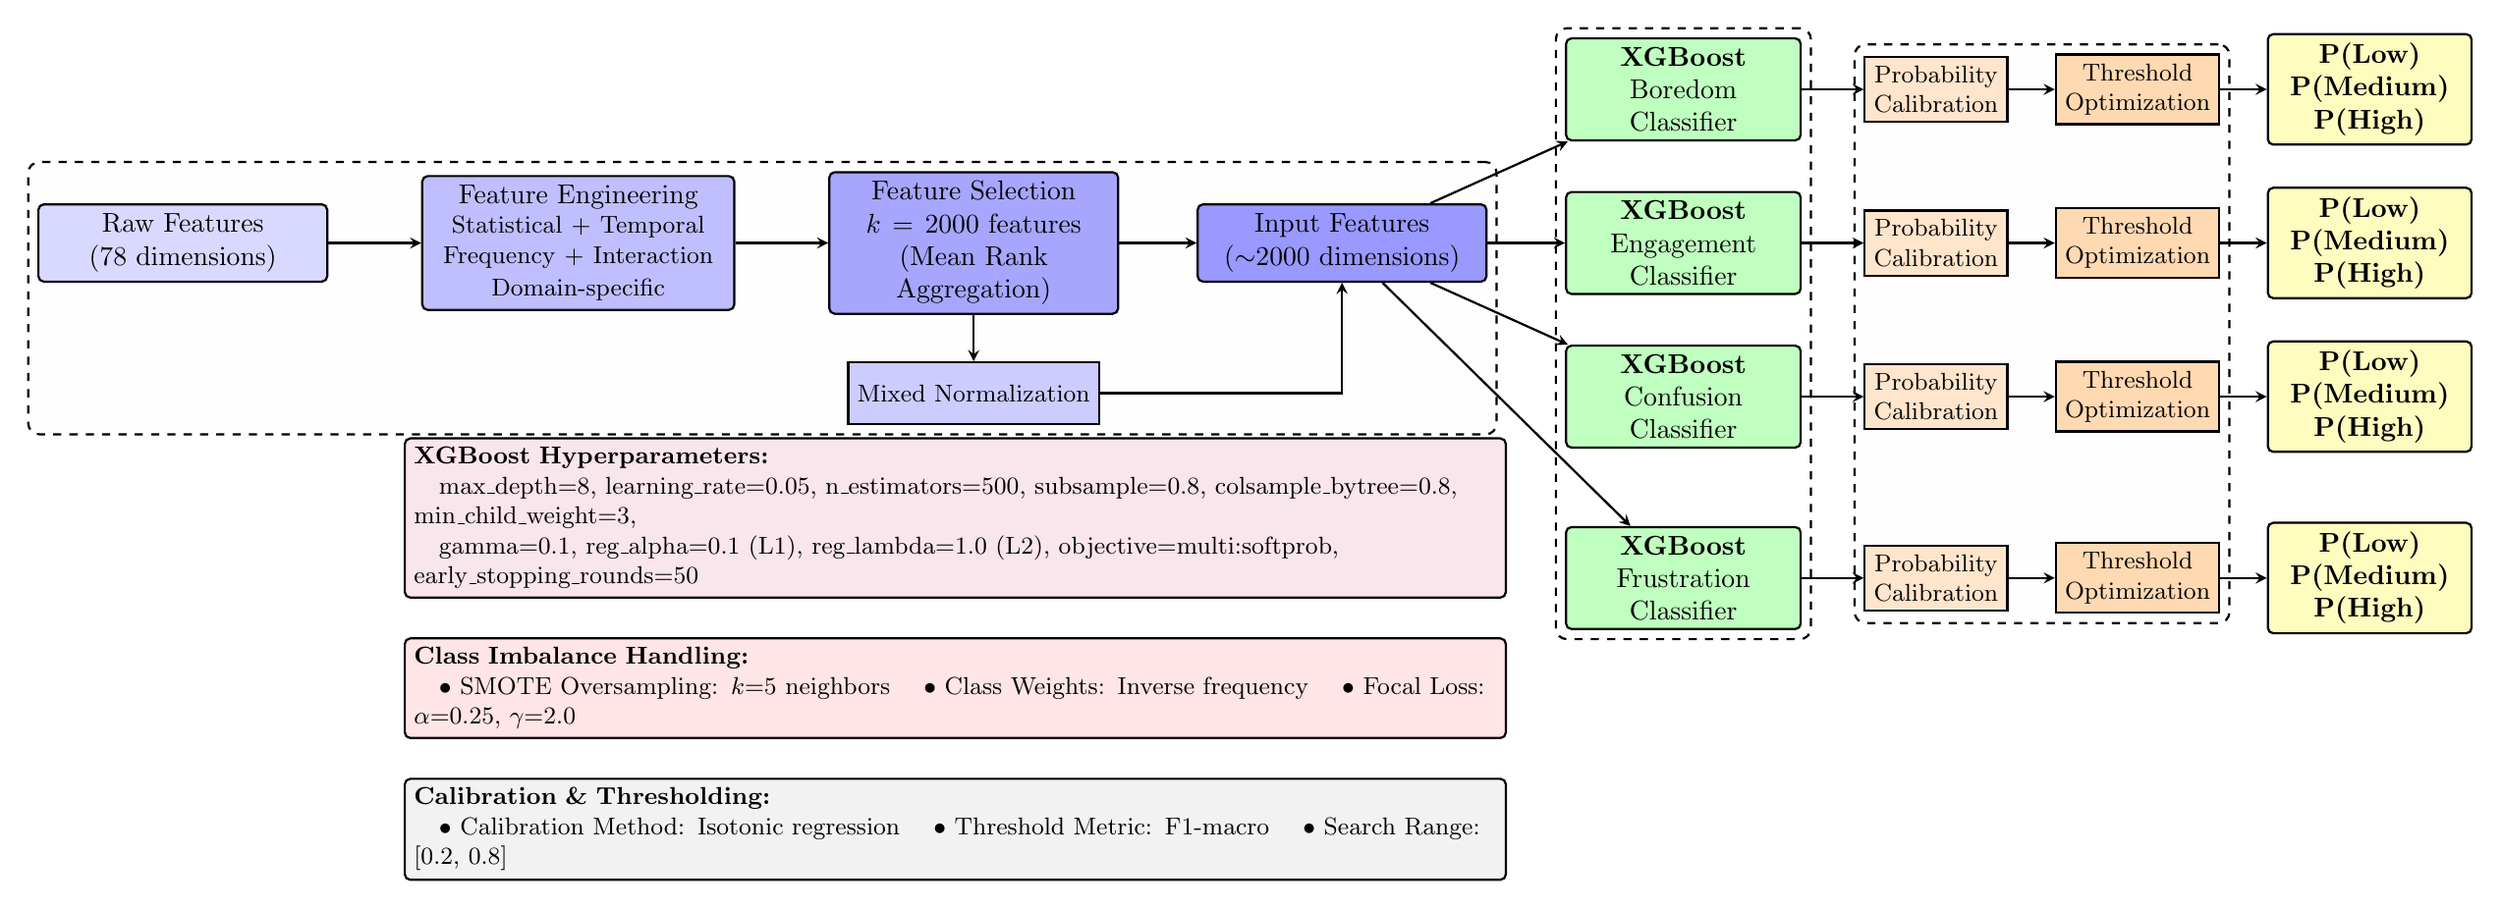
\begin{tikzpicture}[
      node distance=12mm and 8mm,
      box/.style={rectangle, draw, thick, align=center, minimum height=10mm, rounded corners=2pt},
      smallbox/.style={rectangle, draw, thick, align=center, minimum height=8mm, font=\small},
      arrow/.style={->, thick, >=stealth},
      group/.style={draw, dashed, thick, rounded corners, fill opacity=0.1},
      label/.style={font=\bfseries\small}
    ]

    % ============ INPUT PIPELINE ============
    % Raw Input
    \node[box, fill=blue!15, text width=3.5cm] (raw) {Raw Features\\(78 dimensions)};

    % Feature Engineering
    \node[box, fill=blue!25, right=1.2cm of raw, text width=3.8cm] (feng) {Feature Engineering\\{\small Statistical + Temporal\\Frequency + Interaction\\Domain-specific}};

    % Feature Selection
    \node[box, fill=blue!35, right=1.2cm of feng, text width=3.5cm] (fsel) {Feature Selection\\$k=2000$ features\\(Mean Rank Aggregation)};

    % Normalization
    \node[smallbox, fill=blue!20, below=0.6cm of fsel] (norm) {Mixed Normalization};

    % Input to Models
    \node[box, fill=blue!40, right=1cm of fsel, text width=3.5cm] (input) {Input Features\\($\sim$2000 dimensions)};

    % Arrows for preprocessing
    \draw[arrow] (raw) -- (feng);
    \draw[arrow] (feng) -- (fsel);
    \draw[arrow] (fsel) -- (input);
    \draw[arrow] (fsel) -- (norm);
    \draw[arrow] (norm) -| ($(input.south)-(0,0.3)$) -- (input.south);

    % ============ CLASSIFIERS ============
    % 4 XGBoost Classifiers
    \node[box, fill=green!25, above right=0.8cm and 1cm of input, text width=2.8cm] (bore) {\textbf{XGBoost}\\Boredom Classifier};
    \node[box, fill=green!25, right=1cm of input, text width=2.8cm] (enga) {\textbf{XGBoost}\\Engagement Classifier};
    \node[box, fill=green!25, below right=0.8cm and 1cm of input, text width=2.8cm] (conf) {\textbf{XGBoost}\\Confusion Classifier};
    \node[box, fill=green!25, below=1cm of conf, text width=2.8cm] (frus) {\textbf{XGBoost}\\Frustration Classifier};

    % Arrows to classifiers
    \draw[arrow] (input) -- (bore);
    \draw[arrow] (input) -- (enga);
    \draw[arrow] (input) -- (conf);
    \draw[arrow] (input) -- (frus);

    % ============ POST-PROCESSING ============
    % Calibration
    \node[smallbox, fill=orange!20, right=0.8cm of bore] (cal1) {Probability\\Calibration};
    \node[smallbox, fill=orange!20, right=0.8cm of enga] (cal2) {Probability\\Calibration};
    \node[smallbox, fill=orange!20, right=0.8cm of conf] (cal3) {Probability\\Calibration};
    \node[smallbox, fill=orange!20, right=0.8cm of frus] (cal4) {Probability\\Calibration};

    \draw[arrow] (bore) -- (cal1);
    \draw[arrow] (enga) -- (cal2);
    \draw[arrow] (conf) -- (cal3);
    \draw[arrow] (frus) -- (cal4);

    % Threshold Optimization
    \node[smallbox, fill=orange!30, right=0.6cm of cal1] (thresh1) {Threshold\\Optimization};
    \node[smallbox, fill=orange!30, right=0.6cm of cal2] (thresh2) {Threshold\\Optimization};
    \node[smallbox, fill=orange!30, right=0.6cm of cal3] (thresh3) {Threshold\\Optimization};
    \node[smallbox, fill=orange!30, right=0.6cm of cal4] (thresh4) {Threshold\\Optimization};

    \draw[arrow] (cal1) -- (thresh1);
    \draw[arrow] (cal2) -- (thresh2);
    \draw[arrow] (cal3) -- (thresh3);
    \draw[arrow] (cal4) -- (thresh4);

    % ============ OUTPUT ============
    % Output nodes - 3 classes (Low, Medium, High)
    \node[box, fill=yellow!25, right=0.6cm of thresh1, text width=2.4cm] (out1) {\textbf{P(Low)}\\\textbf{P(Medium)}\\\textbf{P(High)}};
    \node[box, fill=yellow!25, right=0.6cm of thresh2, text width=2.4cm] (out2) {\textbf{P(Low)}\\\textbf{P(Medium)}\\\textbf{P(High)}};
    \node[box, fill=yellow!25, right=0.6cm of thresh3, text width=2.4cm] (out3) {\textbf{P(Low)}\\\textbf{P(Medium)}\\\textbf{P(High)}};
    \node[box, fill=yellow!25, right=0.6cm of thresh4, text width=2.4cm] (out4) {\textbf{P(Low)}\\\textbf{P(Medium)}\\\textbf{P(High)}};

    \draw[arrow] (thresh1) -- (out1);
    \draw[arrow] (thresh2) -- (out2);
    \draw[arrow] (thresh3) -- (out3);
    \draw[arrow] (thresh4) -- (out4);

    % ============ GROUPS ============
    \begin{scope}[on background layer]
      % Preprocessing group
      \node[group, fill=blue!5, fit=(raw) (feng) (fsel) (norm) (input), label={[label, above=0.2cm]above:Preprocessing Pipeline}] (preproc) {};

      % XGBoost models group
      \node[group, fill=green!5, fit=(bore) (enga) (conf) (frus), label={[label, above=0.1cm]above:4 Independent XGBoost Classifiers}] (xgb) {};

      % Post-processing group
      \node[group, fill=orange!5, fit=(cal1) (cal2) (cal3) (cal4) (thresh1) (thresh2) (thresh3) (thresh4), label={[label, above=0.1cm]above:Post-Processing}] (post) {};
    \end{scope}

    % ============ TRAINING COMPONENTS (below) ============
    \node[box, fill=purple!10, below=2cm of input, xshift=-5cm, text width=14cm, align=left, font=\small] (params) {
      \textbf{XGBoost Hyperparameters:} \\
      \quad max\_depth=8, learning\_rate=0.05, n\_estimators=500, subsample=0.8, colsample\_bytree=0.8, min\_child\_weight=3, \\
      \quad gamma=0.1, reg\_alpha=0.1 (L1), reg\_lambda=1.0 (L2), objective=multi:softprob, early\_stopping\_rounds=50
    };

    \node[box, fill=red!10, below=0.5cm of params, text width=14cm, align=left, font=\small] (imbalance) {
      \textbf{Class Imbalance Handling:} \\
      \quad $\bullet$ SMOTE Oversampling: $k$=5 neighbors \quad $\bullet$ Class Weights: Inverse frequency \quad $\bullet$ Focal Loss: $\alpha$=0.25, $\gamma$=2.0
    };

    \node[box, fill=gray!10, below=0.5cm of imbalance, text width=14cm, align=left, font=\small] (misc) {
      \textbf{Calibration \& Thresholding:} \\
      \quad $\bullet$ Calibration Method: Isotonic regression \quad $\bullet$ Threshold Metric: F1-macro \quad $\bullet$ Search Range: [0.2, 0.8]
    };

  \end{tikzpicture}
  \caption{XGBoost Model Architecture for Multi-Task Affective State Recognition. The system processes 78 raw features through feature engineering ($\sim$2000D), trains 4 independent XGBoost classifiers (one per affective state), and applies probability calibration and threshold optimization to output 3-class probabilities (Low/Medium/High) for each state.}
  \label{fig:xgboost_architecture}
\end{figure}

\end{document}
